\chapter{Production of Quarkonia at the LHC}
\label{sec:review}
\chaptermark{Review}
The Standard Model (SM) is the theory which describes the electromagnetic, weak
and strong interactions between elementary particles. The model describes a
wide variety of subatomic phenomena involving known elementary particles and
has been confirmed with high precision measurements. Quantum Chromodynamics 
(QCD), the part of the SM describing strong interactions, originated from 
the quark model started in the 1960s\cite{GellMann:1964nj,Zweig:1981pd}, few
years before the experimental confirmation of the existence of quarks. Quarks are 
the only elementary particles which are subject to the strong interaction. 
Because of a phenomenon called color confinement, they are
never been directly observed,  but can be found within composite particles
called hadrons. There are two types of hadrons named as baryons (qqq), made of
three quarks or anti-quarks, and mesons ($q\bar{q}$), made of a quark 
anti-quark pair. There are 6 types of quarks, each with a different {\em{flavour}}: 
up (u), down (d), strange (s), charm (c), bottom or beauty (b), top or
truth (t).

Quarkonia, i.e. bound states of heavy quark-antiquark pairs, are particularly
interesting in this context, since they provide a testing ground of QCD in a
relatively simple and calculable environment. Moreover the production of
quarkonia at LHC represents an interesting check of production mechanisms and
models. Toponia ($t\bar{t}$) states are expected to decay very quickly, due to
the heavy top quark mass, and have never been observed. The experimentally
established quarkonia consist therefore of charmonium ($c\bar{c}$) and
bottomonium ($b\bar{b}$) states.

The $\jpsi$ meson, made up of $c\bar{c}$, was the first observed quarkonium
state\cite{PhysRevLett.33.1404}, with a mass around 3.1\gevcc and narrow width.
The analogous bound state in the $b$ sector was established with the
observation of the $\Upsilon(1S)$ meson in 1977 \cite{Herb:1977ek}. There is a
wide variety of quarkonium states, each differing from other by quantum
numbers: the principal quantum number ($n$), the relative angular momentum
between the quarks ($L$), the spin combination of the two quarks ($S$) and the
total angular momentum ($J$) with $J = L + S$. The spectroscopic notation
$J^{PC}$ is often used, where $P$ and $C$ are parity and
charge conjugation values, respectively. For the quarkonium states, they are
defined as $P=(-1)^{L+1}$ and $C=(-1)^{L+S}$. Table \ref{tab:quarkonium} shows
the properties of some quarkonium states.

\begin{table}[H]
\centering
\caption{Properties of quarkonium states relevant in this thesis.}
% \resizebox{.75\textwidth}{!}{
\begin{tabular}{lccl}\toprule
Meson & $n^{2S+1} L_J$ &  $J^{PC}$ & Mass (\mevcc)\\
\midrule
$\eta_c(1S)$    & $1^1 S_0$ & $0^{-+}$ & $2980.4 \pm 1.2$ \\
$\jpsi(1S)$    & $1^3 S_1$ & $1^{--}$ & $3096.916 \pm 0.011$ \\
$\chi_{c0}(1P)$ & $1^3 P_0$ & $0^{++}$ & $3414.75 \pm 0.31$ \\
$\chi_{c1}(1P)$ & $1^3 P_1$ & $1^{++}$ & $3510.66 \pm 0.07$ \\
$h_{c}(1P)$     & $1^3 P_1$ & $1^{++}$ & $3525.93 \pm 0.27$ \\
$\chi_{c2}(1P)$ & $1^3 P_2$ & $2^{++}$ & $3556.20 \pm 0.09$ \\
$\eta_{c}(2S)$  & $2^1 S_0$ & $0^{-+}$ & $3637 \pm 4$ \\
$\psi(2S)$      & $2^3 S_1$ & $1^{--}$ & $3686.09 \pm 0.04$ \\
\midrule
$\eta_b$        & $1^1 S_0$ & $0^{-+}$ & $9388.9 \pm 2.5 \pm 2.7$ \\
$\Upsilon(1S)$  & $1^3 S_1$ & $1^{--}$ & $9460.30 \pm 0.26$\\
$\chi_{b0}(1P)$ & $1^3 P_0$ & $0^{++}$ & $9859.44 \pm 0.42 \pm 0.31$ \\
$\chi_{b1}(1P)$ & $1^3 P_1$ & $1^{++}$ & $9892.78 \pm 0.26 \pm 0.31$ \\
$\chi_{b2}(1P)$ & $1^3 P_2$ & $2^{++}$ & $9912.21 \pm 0.26 \pm 0.31$ \\
$\Upsilon(2S)$  & $2^3 S_1$ & $1^{--}$ & $10023.26 \pm 0.31$ \\
$\chi_{b0}(2P)$ & $2^3 P_0$ & $0^{++}$ & $10232.5 \pm 0.4 \pm 0.5$ \\ 
$\chi_{b1}(2P)$ & $2^3 P_1$ & $1^{++}$ & $10255.46 \pm 0.22 \pm 0.5$ \\ 
$\chi_{b2}(2P)$ & $2^3 P_2$ & $2^{++}$ & $10268.65 \pm 0.22 \pm 0.5$ \\ 
$\Upsilon(3S)$  & $2^3 S_1$ & $1^{--}$ & $10355.2 \pm 0.5$ \\
\bottomrule
\end{tabular}
% }
\label{tab:quarkonium}
\end{table}

\begin{figure}[H]
  \setlength{\unitlength}{1mm}
  \centering
  \resizebox{\textwidth}{!}{
  \begin{picture}(150,80)
  \put(0,0){\includegraphics*[width=150mm, height=80mm]{bottomonium}}
  \put(3,25){\Large \begin{sideways}$m(b\bar{b}) \left[\gevcc\right]$\end{sideways}}
  \end{picture}
  }
\caption{Observed (blue) and theoretically predicted (red) bottomonium states}
\label{fig:bottomonium}
\end{figure} 



Bottomonium states and their quantum numbers are shown
in~\Cref{fig:bottomonium}. The $L = 0$ and $L = 1$ states are respectively
called S-wave and P-wave. For example, the \Y1S and the \chiboneOneP are S-wave and 
P-wave mesons, respectively. The principal quantum number $n$ orders states from lowest to highest
masses, such as for $\Upsilon(nS)$, where $n$ equals to 1, 2, 3 and 4. When the
conditions $L = 1$ and $S = 1$ are satisfied, J takes the value 0, 1 or 2, with the spin-orbit coupling 
causing mass level splitting. Thus,
each \chib states has three sub-states indexed by the value of the quantum
number J. For example, the $\chi_b(1P)$ state has three sub-states $\chi_{bJ}(1P)$,
where J is equal to 0, 1 and 2.

Radiative transitions from one bottomonium state to another with the emission of a photon 
have been observed, with selection rules being the same as for the hydrogen atom energy states. 
The electric dipole is the leading order transition, which changes the relative angular
momentum $\Delta L  = \pm 1$ but not the spin $\Delta S = 0$. The magnetic
dipole transition is next-to-leading order and is therefore suppressed. 
This transition changes the spin $\Delta S = \pm 1$ but not the relative
angular momentum $\Delta L = 0$. The radiative decays exploited in 
this thesis involve the leading order transitions $\chi_b \rightarrow \Upsilon \gamma$. 

\section{The quarkonium mass spectrum}

Many theoretical models have been developed to describe quarkonium systems.
These models can be roughly split in two classes, based respectively on Lattice
QCD calculations and phenomenological approaches. The simplest and most
frequently used phenomenological approach is the {\it non-relativistic
potential model}, an effective theory in which the quark move non-
relativistically inside hadrons. Similarly to the positronium case, the system
is characterized by a typical velocity $v$ given by the strong coupling constant
$\alpha_s$, evaluated at a scale corresponding to the typical size of the bound
state

\begin{equation}
v \sim \alpha_s(1/r^2), r \sim 1/mv
\end{equation}

\noindent Being $v$ larger than $\alpha_s(m^2)$, higher-order corrections to the 
non-relativistic approximation are potentially more important than higher-order
perturbative corrections. So far the theoretical calculations of charmonium and
bottomonium and their spectra measured by many experiments suggest that the
potential of quarkonium possesses a radial dependence of an approximately
Coulomb form at small distances due to gluon exchange

\begin{equation}
V(r) \sim -{\frac{4}{3}}{\frac{\alpha_s(1/r^2)}{r}} \quad (r\rightarrow 0)
\end{equation}
\noindent and is confining at large distances due to the increasing strength 
of the coupling
\begin{equation}
V(r) \sim kr \quad (r\rightarrow \infty)
\end{equation}

\noindent where k is the string tension and the factor of 4/3 arises from the
SU(3) colour factors. Several models have been widely used for explaining the
quarkonium spectroscopy. Although these potentials have different asymptotic
behaviours at small and large distances, they coincide with each other in the
region $0.1 fm < r <1 fm$, where $r$ is the average distance between heavy quarks
in the bound systems. Experimental measurements can be used as inputs to
understand the exact shape of the strong potential. For instance, the Cornell
model

\begin{equation}
V_C(r) = -{\frac{4}{3}}{\frac{\alpha_s}{r}} + {\frac{r}{a^2}} + c_0
\end{equation}  

\noindent describes the fine and hyperfine structures of charmonium levels in the leading
non-relativistic treatment. By using charmonium data, the coefficients are
determined to be $\alpha_s = 0.36$, $a=2.34 \gev^{-1}$, $c_0 = -0.25 \gev$, $m_c
= 1.84\gev$.

Energy levels and wave functions of the quarkonium system are obtained by solving 
the non-relativistic Schr\"odinger equation in terms of the constituent masses and the 
potential function. The wavefunction, $\Psi(r) = \Psi_{nL}(r)Y_{Lm}(\theta,\phi)$, with 
$\Psi_{nL}(r)$ and $Y_{Lm}(\theta,\phi)$ being the radial and orbital parts of the wavefunction, 
gives predictions of quarkonium properties. The radial wavefunctions of the $\jpsi$ and 
$\psi(2S)$ systems from various potential models are shown in \Cref{fig:psipot}. 
Up to 30\% differences can be noticed at small values of $r$. 

\begin{figure}
\center
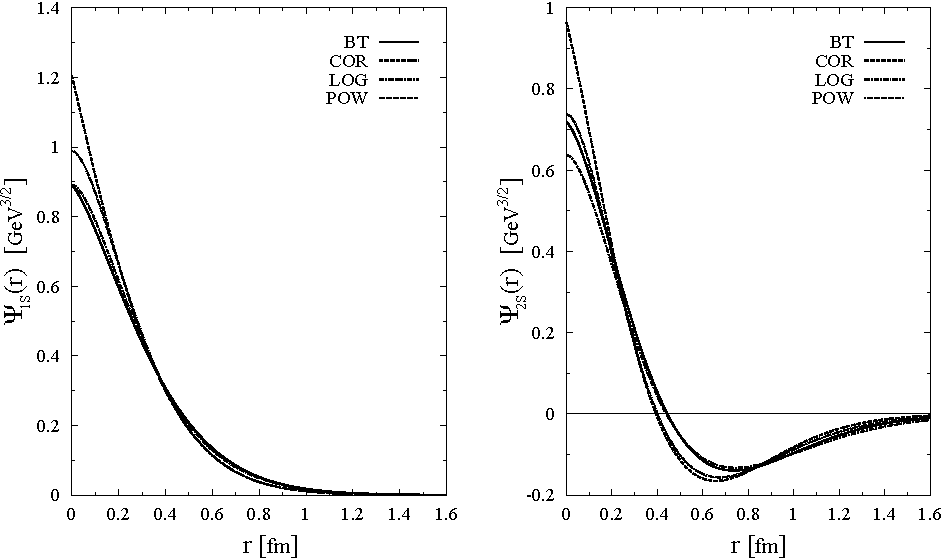
\includegraphics[width=\textwidth]{figs/review/psipot}
\caption{Radial Wave functions for the $\jpsi$ (left) and $\psi(2S)$ (right) for different 
potential models: Buchm\"uller and Tye (BT), Cornell (COR), Logarihmic (LOG) and Power (POW). }
\label{fig:psipot} 
\end{figure} 


\section{Quarkonium production}

The production of quarkonium states can be split in two parts: the production
of a heavy quark-antiquark pair in the regime of perturbative QCD, and the
formation of a bound state, which is driven by non-perturbative QCD. Many
theoretical models have been proposed to interpret the quarkonium production
rates measured by experiments.

\subsection{Colour Singlet Model}

\begin{figure}
\center
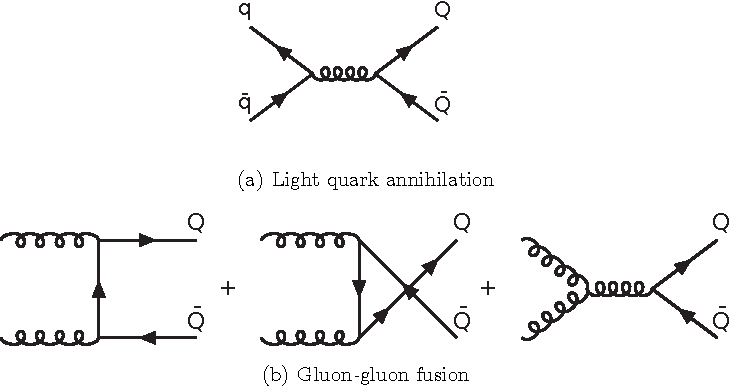
\includegraphics[width=\textwidth]{figs/review/heavy}
\caption{Leading-order Feynman diagrams for heavy quark production\cite{Ellis:318585}}
\label{fig:heavy} 
\end{figure} 


The leading order diagrams for the production of a $Q\bar{Q}$ pair are shown in
\Cref{fig:heavy}. Quark-antiquark annihilation produces a pair in an octet
state, while gluon-gluon fusion can give a  pair in either a singlet or an
octet state, mainly the latter. The Colour Singlet Model (CSM)\cite{Humpert:171969}
assumes that a given quarkonium state can only be produced from a heavy quark
pair with the same quantum numbers. In particular, the quark pair must have
the same spin and colour state as the final quarkonium state, i.e. colour
neutral. The formation of a quarkonium bound state is parameterised by
non-perturbative theory in the CSM into one single term, assuming the constituent
quarks are at rest in the meson frame ({\it{static approximation}}). The 
short-distance cross section for the whole process can be written as

\begin{equation}
d{\hat{\sigma}}(ij\rightarrow H + X) = d{\hat{\sigma}}(ij\rightarrow Q{\bar{Q}}\left[n^{2S+1}L_J\right] + X) 
|\Psi^{(k)}_{nL}(0)|^2
\end{equation}

\noindent where the radial wave functions at the origin can be extracted from
the non-relativistic potential models. The wave function $\Psi_{nL}(0)$ is zero
for P-wave states (e.g. $\chi$ states). For these states, the next term in the
amplitude expansion $\Psi'_{nL}(0)$, is used. At order $\alpha_s^2$ there is
only one diagram that contributes for the production of $\eta$ and $\chi$
states. Due to C-parity conservation, the production of $J/\psi$ and $\Upsilon$
states from gluon fusion at leading order is forbidden, and it is described by
an $\alpha_s^3$ term in the CSM. Therefore, this model predicts that the
prompt $\jpsi$ production cross section is lower than the $\chi_c$ one, which is in
disagreement with data~\cite{Schuler:1994hy}.

\subsection{Colour Octet Model}

The Colour Octet Model (COM)~\cite{Braaten:1993rw,Bodwin:1994jh} extends the CSM calculation and
mitigates its shortcomings when compared to data. The COM allows the heavy
quark pair produced in the hard process to have different quantum numbers and
evolve into a given quarkonium state through radiation of soft gluons during
hadronisation. The perturbative hard process is separated from the non-
perturbative dynamics, in which the heavy bound states are inherently non-
relativistic. The latter process can be described in the formalism of NRQCD
(non-relativistic QCD) where a production cross section of a heavy quarkonium
state H can be expressed as

\begin{equation}
d\sigma ( i j \rightarrow H + X ) = \sum_{\cal{Q}} d{\hat{\sigma}}(Q{\bar{Q}}[{\cal{Q}}] + X') 
\langle O^H({\cal{Q}})\rangle
\end{equation}

\noindent where $d{\hat{\sigma}}(Q{\bar{Q}}[{\cal{Q}}] + X')$ describes the
short-distance production of a  $Q{\bar{Q}}$ pair, $Q{\bar{Q}}[{\cal{Q}}]$ is
the Fock state component of the quarkonium wave function in the colour, spin,
and angular momentum state ${\cal{Q}} =^{2S+1} L_J^{[1,8]}$, and
$\langle O^H({\cal{Q}})\rangle$ is the vacuum expectation value of the operator describing
the hadronisation into the final state H. Using NRQCD velocity scaling rules,
the quarkonium state can be expanded in terms of the heavy quark velocity $v$,
for example, the S-wave vector meson can schematically be written as:

\begin{equation}
\begin{split}
|\psi_Q\rangle = O(1)|Q{\bar{Q}}[^3S_1^{(1)}]   \rangle + O(v)|Q{\bar{Q}}[^3P_J^{(8)}] g\rangle + O(v^2)|Q{\bar{Q}}[^1S_0^{(8)}]    g\rangle + \\
+ O(v^2)|Q{\bar{Q}}[^3S_1^{(1,8)}]  gg\rangle + O(v^2)|Q{\bar{Q}}[^3D_J^{(1,8)}]\rangle + \ldots
\end{split}
\end{equation}   

\noindent where the lowest order in $v$ corresponds to the CSM case. For P-wave
quarkonia, contributions from colour-octet S-wave states are at the same order
in $v$ as those from the leading colour-singlet P-wave states. Although the
parameters of the non-perturbative matrix elements in NRQCD are free, they are
independent of the hard process, therefore they can be extracted from multiple
experiments. The application of NRQCD in the COM model provides an acceptable
description of the differential $\jpsi$ production cross section to CDF data.
For the $\Upsilon$ production, corrections at low $p_T$ are required.

\section{Production of \chib mesons at LHC}

Recently ATLAS~\cite{Aad:2011ih}, D0~\cite{Abazov:2012gh} and
LHCb~\cite{LHCb-CONF-2012-020} 
observed radial excitations of the P-wave $\chi_b$ states in radiative
transitions to the S-wave $\Upsilon$ states. Also, the $\chi_b(3P)$ states 
were observed for the first time, even though the invariant mass resolution was
not adequate to separate the different spin sub-states.

The main contribution to the production processes at the \tev scale is due to
gluon fusion. As seen before, the production of quarkonia can be factorized
into two parts, namely the determination of the transverse momentum of the
final state using the initial parton distribution function, and the
hadronization process. Vanishing production cross-sections in gluon fusion for
$|^3 S_1\rangle (1^{--})$ states, due to charge parity conservation, can be avoided
by additional gluon emission in the final state. However, the predicted high
$p_T$ spectrum is in contradiction with experimental data. For P-wave mesons,
it is difficult to obtain the transverse momentum distribution of final states.
In addition, the Landau-Yang theorem forbids the production of axial mesons
such as the $|^3P_1\rangle$ state, from two massless gluons.

The authors of Ref.~\cite{Likhoded:2012hw} showed that these problems can be overcome
by considering next to leading order terms, namely the emission of a single
hard gluon as can be seen in \Cref{fig:chibprod_fig1}.
\begin{figure}
\center
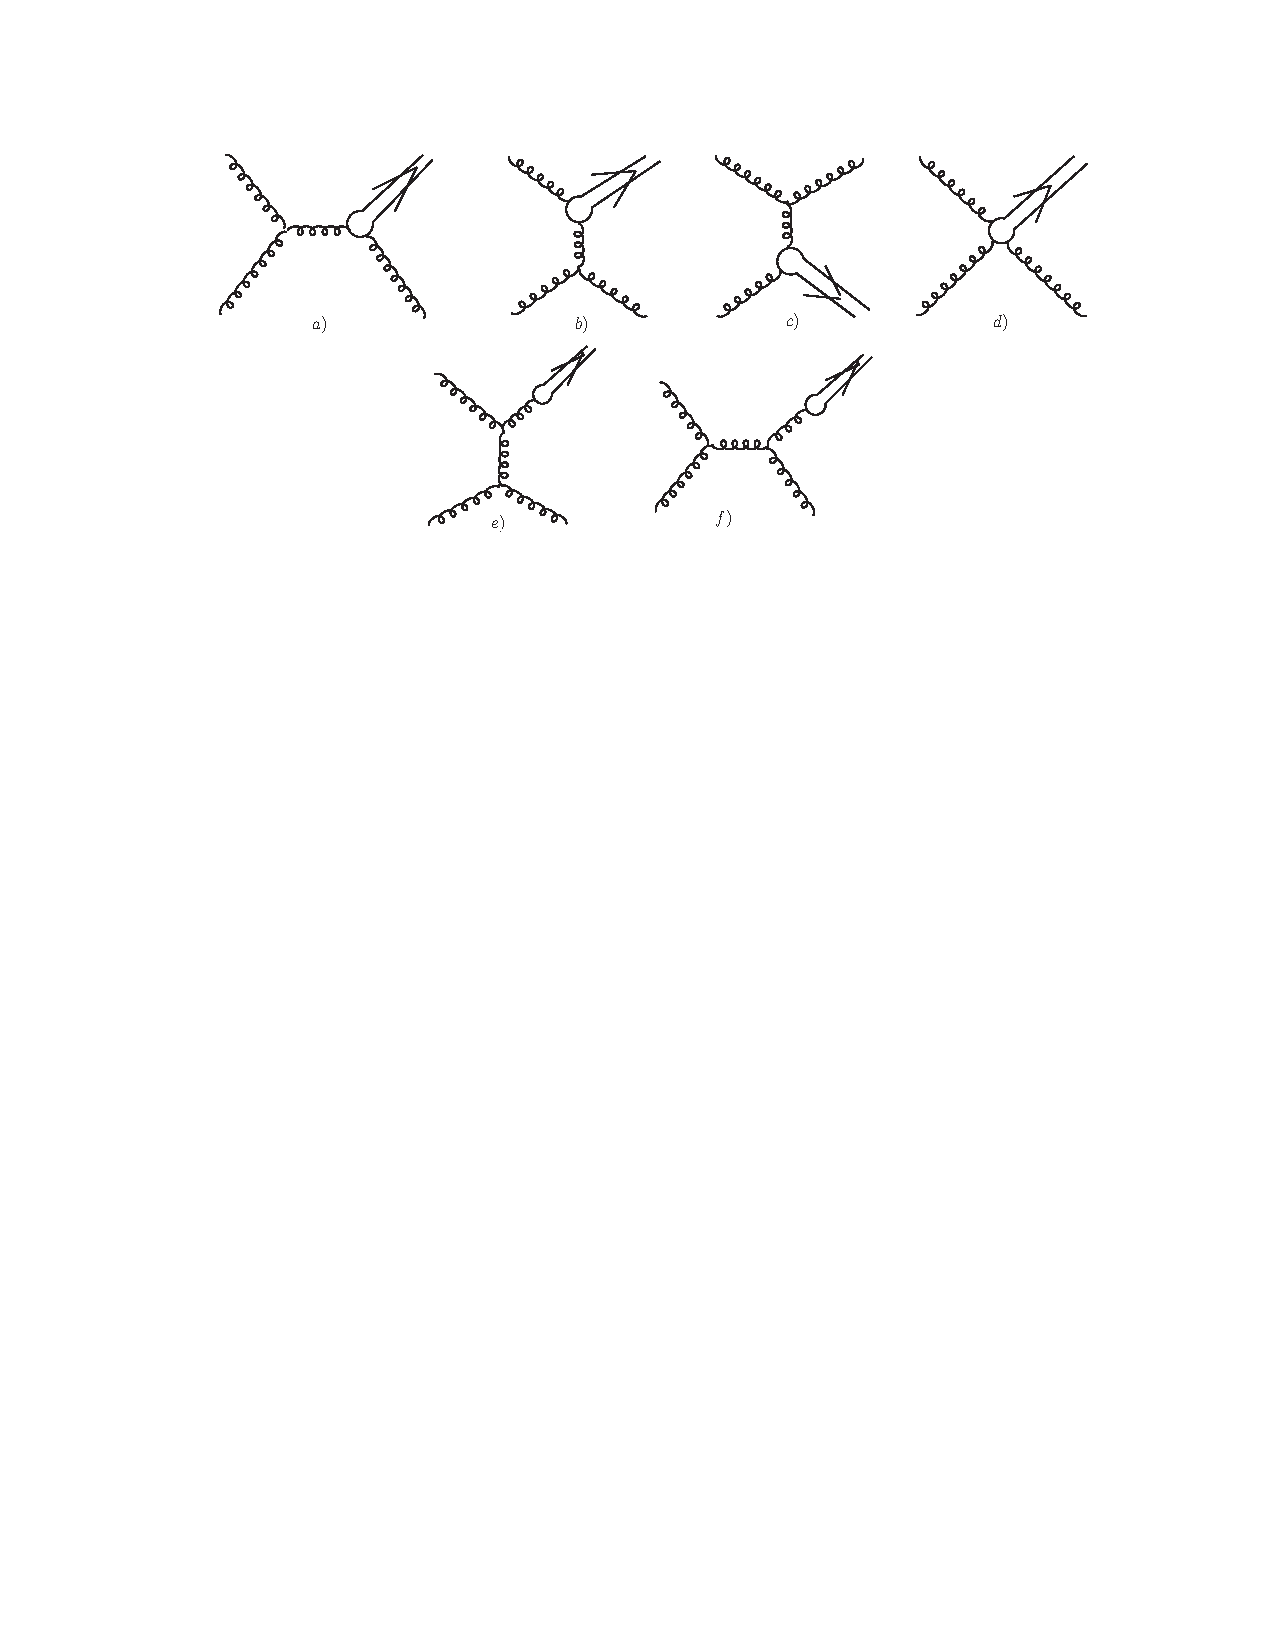
\includegraphics[width=.75\textwidth]{figs/review/chibprod_fig1}
\caption{From Ref.~\cite{Likhoded:2012hw}: Feynman diagrams of the $gg\rightarrow \chi_b g$ NLO 
process. The diagrams in the top row give both CS and CO contributions, the ones in the 
bottom row result only in CO contributions.}
\label{fig:chibprod_fig1} 
\end{figure} 
In this way, all three P-wave states can be produced. 
The observed $p_T$ dependence of the production cross-section is well reproduced by 
the color singlet contribution. However, the absolute normalization is several time smaller 
than measured. This discrepancy can be solved for the $\chi_c$ spectrum (see \Cref{fig:chibprod_fig2})
by considering color-octet contributions.

\begin{figure}
\center
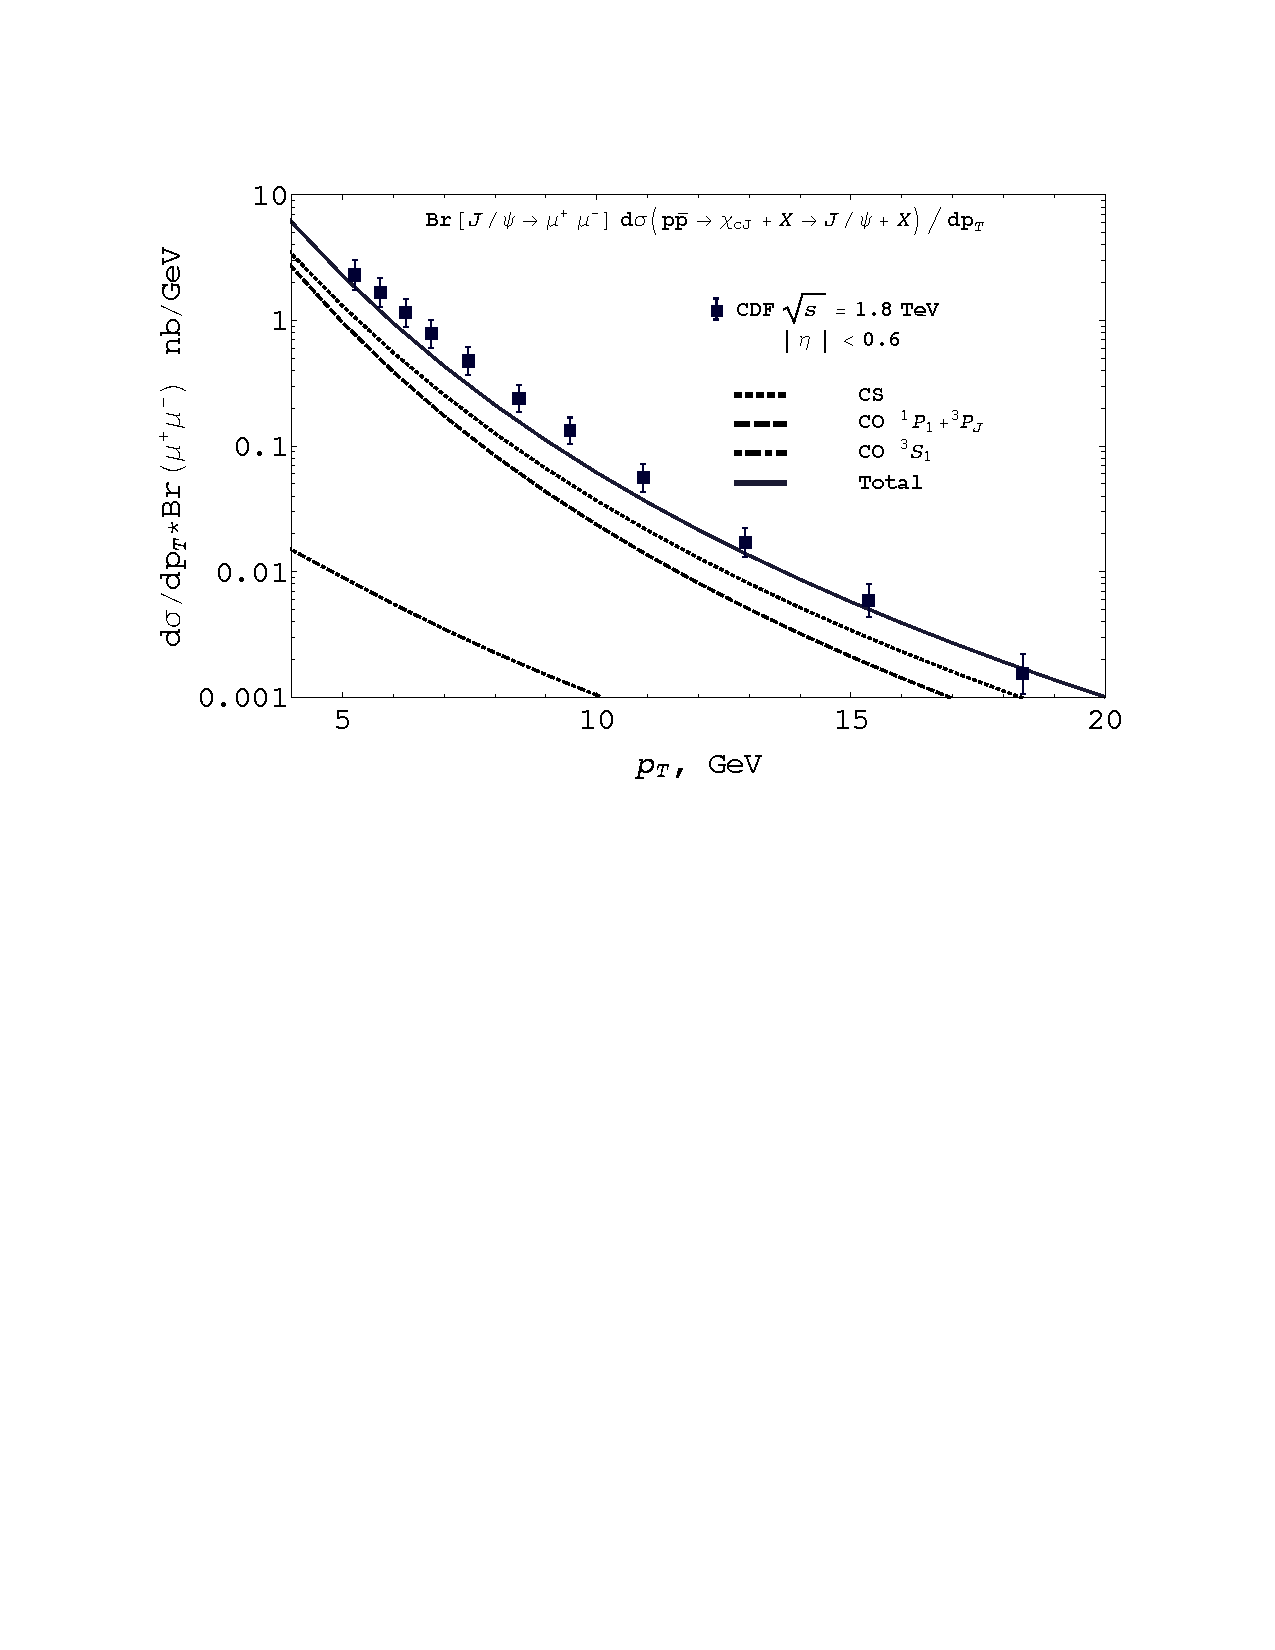
\includegraphics[width=.75\textwidth]{figs/review/chibprod_fig2}
\caption{From~\cite{Likhoded:2012hw}: Differential production cross section for $\chi_c$ mesons, 
as a function of $p_T$. The different lines correspond to CS (dotted), two different CO 
contributions (dashed and dot-dashed), total (solid). Experimental points are taken from a 
CDF report~\cite{Abulencia:2007bra}.}
\label{fig:chibprod_fig2} 
\end{figure} 

\begin{figure}
\center
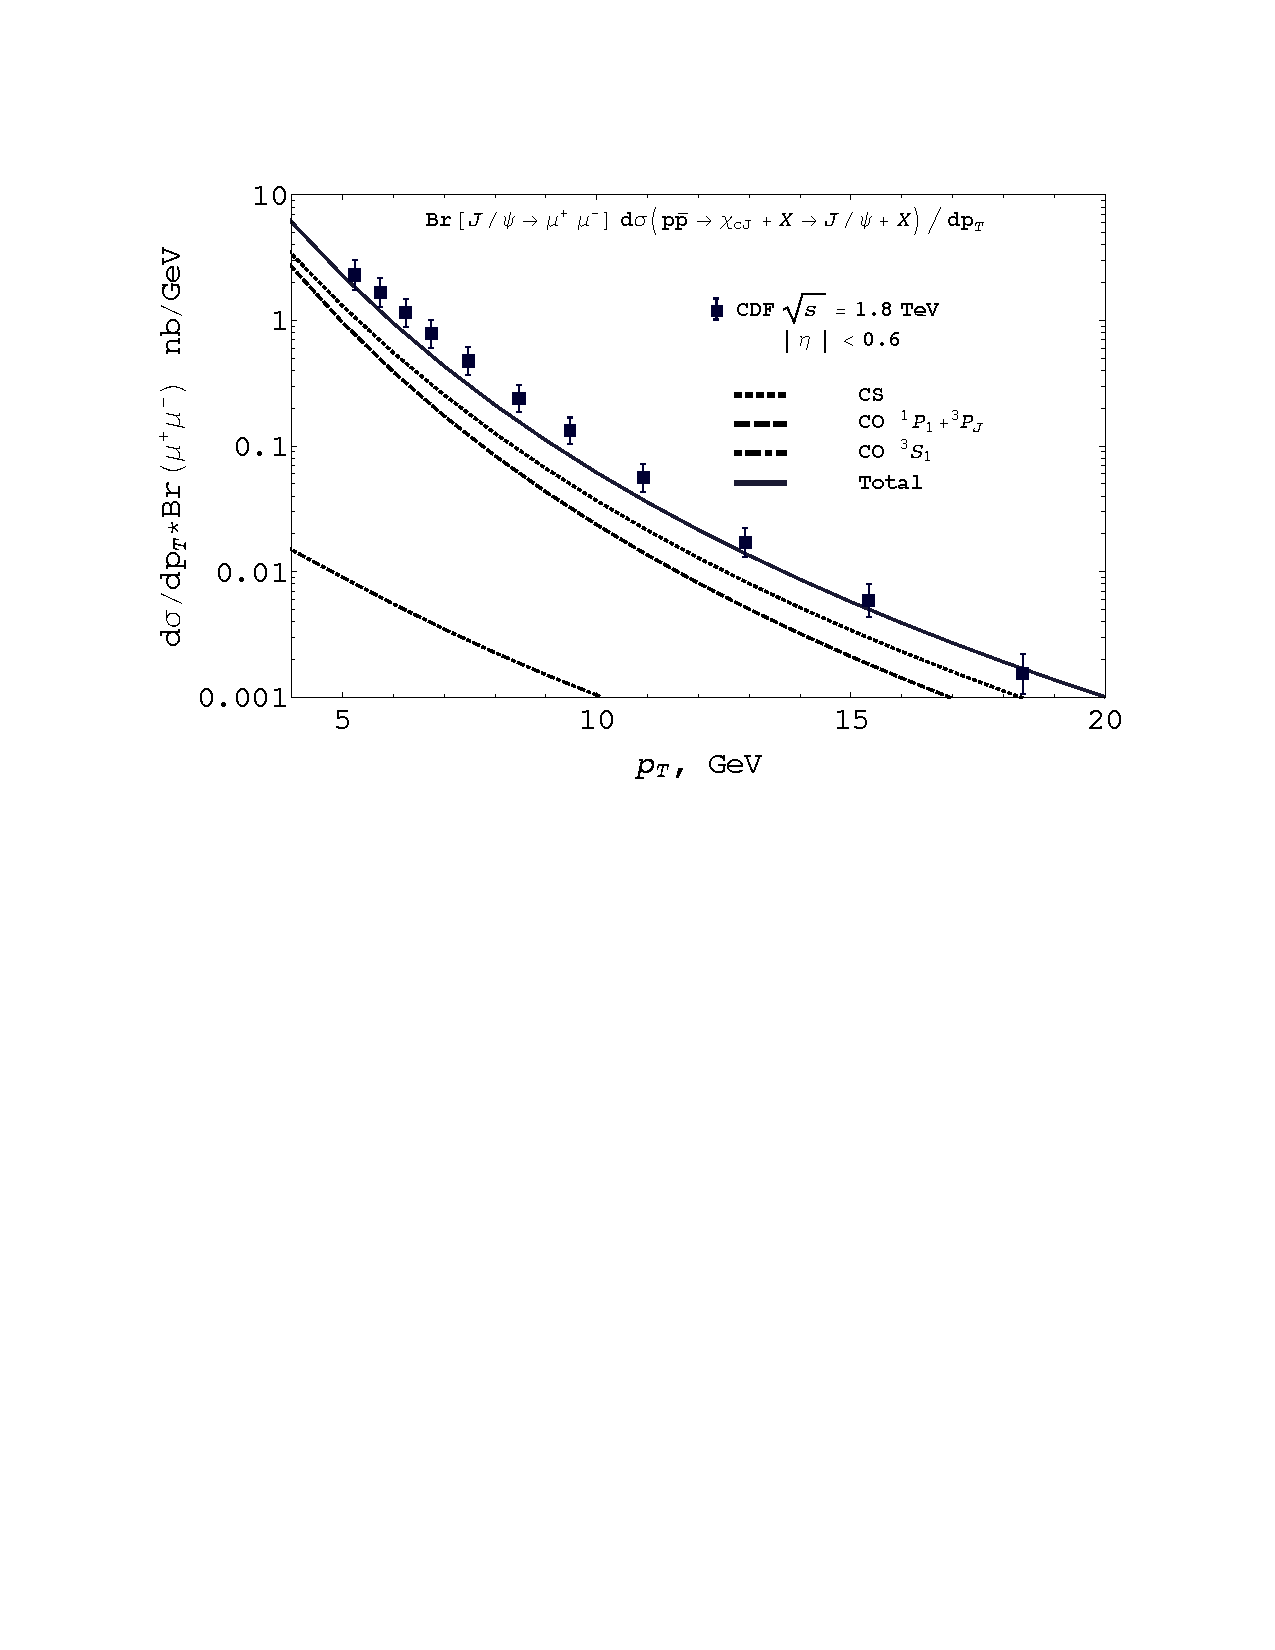
\includegraphics[width=.75\textwidth]{figs/review/chibprod_fig3}
\caption{From Ref.~\cite{Likhoded:2012hw}: Transverse momentum distribution for $\chi_b$ states at 
$\sqs=1.8\tev$.}
\label{fig:chibprod_fig3} 
\end{figure} 

The predicted production cross sections of $\chi_b$ states are given in
\Cref{fig:chibprod_fig3}. The ratio of production cross-sections for $J=2$ and
$J=1$ states as a function of transverse momentum gives a good description of
$\chi_c$ data, see \Cref{fig:frac:ratio}. From that Figure, it is also
interesting to notice that the corresponding ratio for $\chi_b$ mesons, after
rescaling the $p_T$ variable $p_T \rightarrow M_{\chi_c} / M_{\chi_b} p_T
\approx 1/3 p_T$, nicely matches the $\chi_c$ curve. Unfortunately, as we will
see in the following, the invariant mass resolution achieved in this thesis is
not adequate to distinguish the different $\chi_b$ spin states. An approach
based on converted photons might be able to do so in the future, so that these
theoretical predictions can be checked. Compared with other experiments, LHCb
results on this ratio allow to check the predictions in higher $\chib$ rapidity
range.

\begin{figure}[ht]
  \setlength{\unitlength}{1mm}
  \centering
  \resizebox{.75\textwidth}{!}{
  \begin{picture}(75,60)
    %
     \put(0,0){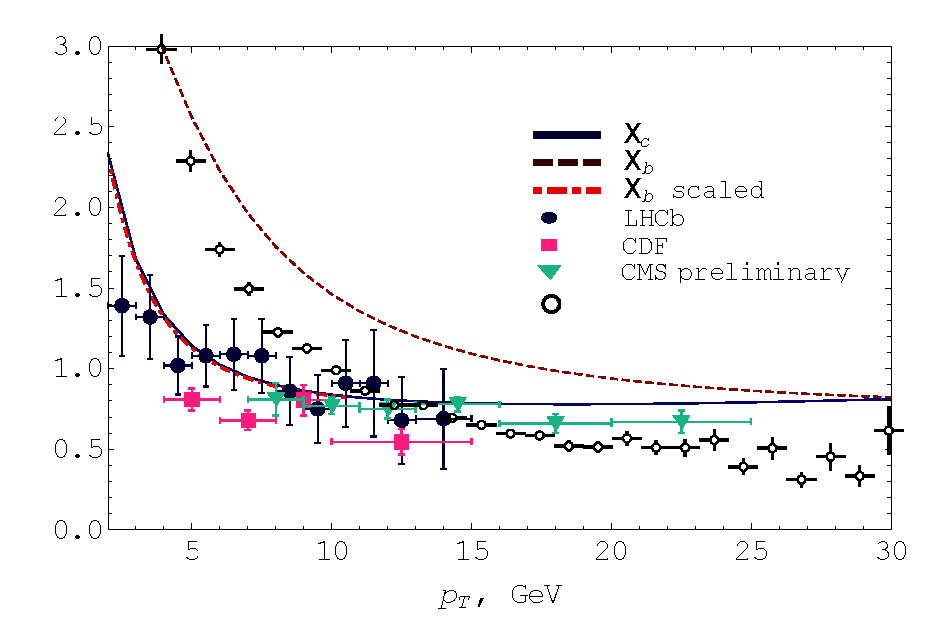
\includegraphics[width=75mm, height=60mm]{ratio/theory}}
     \put(-1,22){\begin{sideways}$\sigma({\chi_2})/\sigma({\chi_1}$)\end{sideways}}
   \end{picture}
  }
  \caption {\small This figure is taken from~\cite{Likhoded:2012hw} and shows
  transverse momentum distributions of the
$d\sigma\left[\chi_{2}\right]/d\sigma[\chi_{1}]$ ratio. Solid and dashed lines
stand for charmonium and bottomonium mesons. The dot-dashed line corresponds to
the rescaled bottomonium ratio:
$\sigma_{b2}/\sigma_{b1}(M_{\chi_c}/M_{\chi_b}p_T)$. The experimental results
for charmonium from LHCb\cite{LHCb-PAPER-2013-028} are shown with dots,
CDF~\cite{Abulencia:2007bra} --- with rectangles, and CMS~\cite{Chatrchyan:2012ub}
--- with triangles.}
  \label{fig:frac:ratio}
\end{figure}




Finally, the production cross sections for different radial excitations of $\chi_b$ states, summed over spin states, 
are predicted and can be compared with experimental measurements. As an example, the authors of Ref.~\cite{Likhoded:2012hw} give
the following prediction for $2 < y  < 4.5$ and $6 < p_T < (s-M^2)/2\sqrt{s} \gevc$:

\begin{equation}
\frac{\sigma^{th}[2P,1S]}{\sigma^{th}[1P,1S]} = (0.29 \pm 0.01^{th} \pm 0.1^{br}) \Bigl| \frac{R'_{2P}}{R'_{1P}}\Bigr|^2, 
\end{equation}

\noindent where $\sigma^{th}[nP,mS]$ is the sum over the possible $\chi_b(nP)$ spin states of the production cross 
section for that state multiplied by its branching fraction for the $\Upsilon(mS)$ decay, $R'_{nP} \sim 1$ is the derivative 
of the $\chi_b(nP)$ state wave function at the origin, the first uncertainty is due to the theoretical model and the second 
is due to the experimental values of the branching fractions.  Predictions for this ratio in the range between 0.14 and 0.4 
have been obtained by using different potential models~\cite{Munz:1996hb,Ebert:2003mu,Anisovich:2005jp,Wang:2009er,Li:2009nr,Hwang:2010iq}. 

A measurement of the ratio of the $\chi_b(3P)$ and $\chi_b(1P)$ production cross sections can be used, with additional assumption, 
to infer the $\chi_b(3P)$ radiative branching fractions into $\Upsilon(1S)$. 

